% !TEX root = ../ResearchBook.tex


\chapter{Integrated Planning for Multiple Types of Locomotive Work Facilities under Location, Routing, and Inventory Considerations}\label{chap:locomotive}
\chaptermark{Planning of Locomotive Facilities} % short chapter name



\section{Problem Description}\label{sec:locomotive:problem}

The assignment of repair, service, and fueling demands to various suitable facilities is determined holistically, and is represented by the solid and dashed arrows in Figure \ref{fig:locomotive:problem}.
\begin{figure}[!ht]
  \centering
    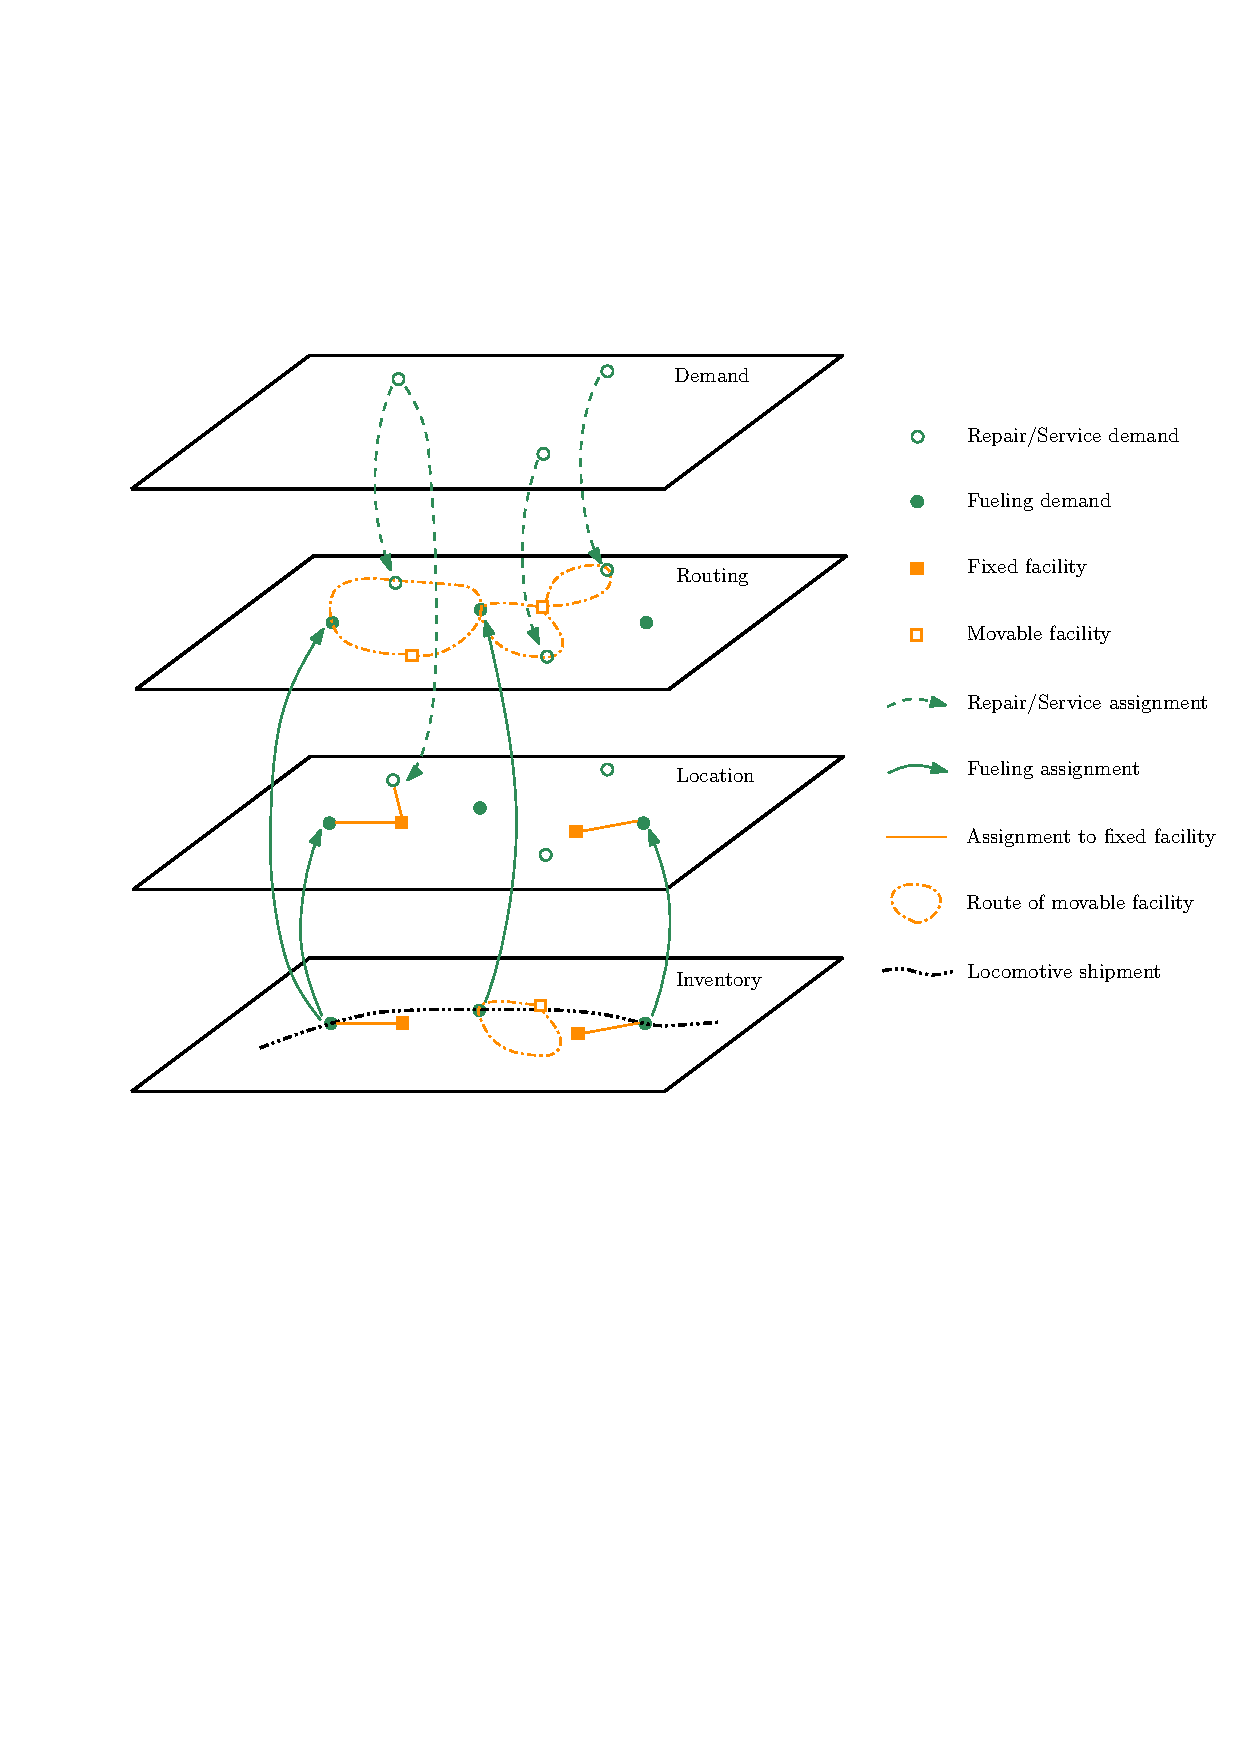
\includegraphics[width=0.75\textwidth]{images_locomotive/Figure1.pdf}
  \caption{The planning problems consist of multiple layers of decisions.} 
  \label{fig:locomotive:problem}
\end{figure}



\section{Model Formulation}\label{sec:locomotive:formulation}

In this section, we present the model formulation of solving the integrated locomotive facility planning problem, with explaination of the network transformation methods in mathematical details.


\subsection{Notation}\label{sec:locomotive:notation}
We first describe the notation used in the model formulation.

\subsubsection{Sets}
\begin{tabular}{ll}  % first type of notation list
    $\mathcal{F}$            & set of fixed facility types.  \\
    $\mathcal{M}$            & set of movable facility types.  \\
    $\mathcal{S}$            & set of work types, excluding fueling.  \\
\end{tabular}

\subsubsection{Parameters} 
\begin{notation}   % second type of notation list
  \item[$F_{n}^{\alpha}$] Annual fixed cost of operating a facility of type $\alpha$ at candidate location $n$.
  \item[$C_{n}^{\alpha}$] Cost of unit capacity at a facility of type $\alpha$ at yard $n$.
  \item[$Q_{n}^{\alpha,\max}$] Maximum (minimum) allowable capacity of facility type $\alpha$ at yard $n$.
\end{notation}

\subsection{Location-Inventory Problem Formulation}\label{sec:locomotive:location-inventory}
Below, we present the formulation for the location-inventory problem.

\subsubsection{Objective}
\begin{align*}
   \text{Minimize} ~ & \sum_{\alpha \in \mathcal{F}\cup\mathcal{M}} \sum_{n\in \mathcal{N}_{\alpha}} x_{n}^{\alpha} F_{n}^{\alpha} + \sum_{\alpha \in \mathcal{F}}\sum_{n\in \mathcal{N}_{\alpha}} q_{n}^{\alpha} C_{n}^{\alpha} + \sum_{l\in \mathcal{M}}\sum_{n\in \mathcal{N}_{l}}\left( h_{n}^{l}\cdot F_{l} + t_{n}^{l}\cdot V_{l} \right) \\
  & + \sum_{r\in\mathcal{R}}\sum_{s\in \mathcal{S}_{r}}E_{r}\left[ h_{r}^{s}\sum_{n\in \mathcal{N}}\left(G_{r,s}^{n}\cdot C_n\right) + p_{r}^s\sum_{n\in \mathcal{N}}\left(G_{r,s}^n\cdot C_{n,0}\right) \right]
\end{align*}



\section{Solution Approach}\label{sec:locomotive:algorithm}

\begin{figure}[!htbp]
\centering
    \subfigure[Transformation for train network \citep{xie2014planning}]{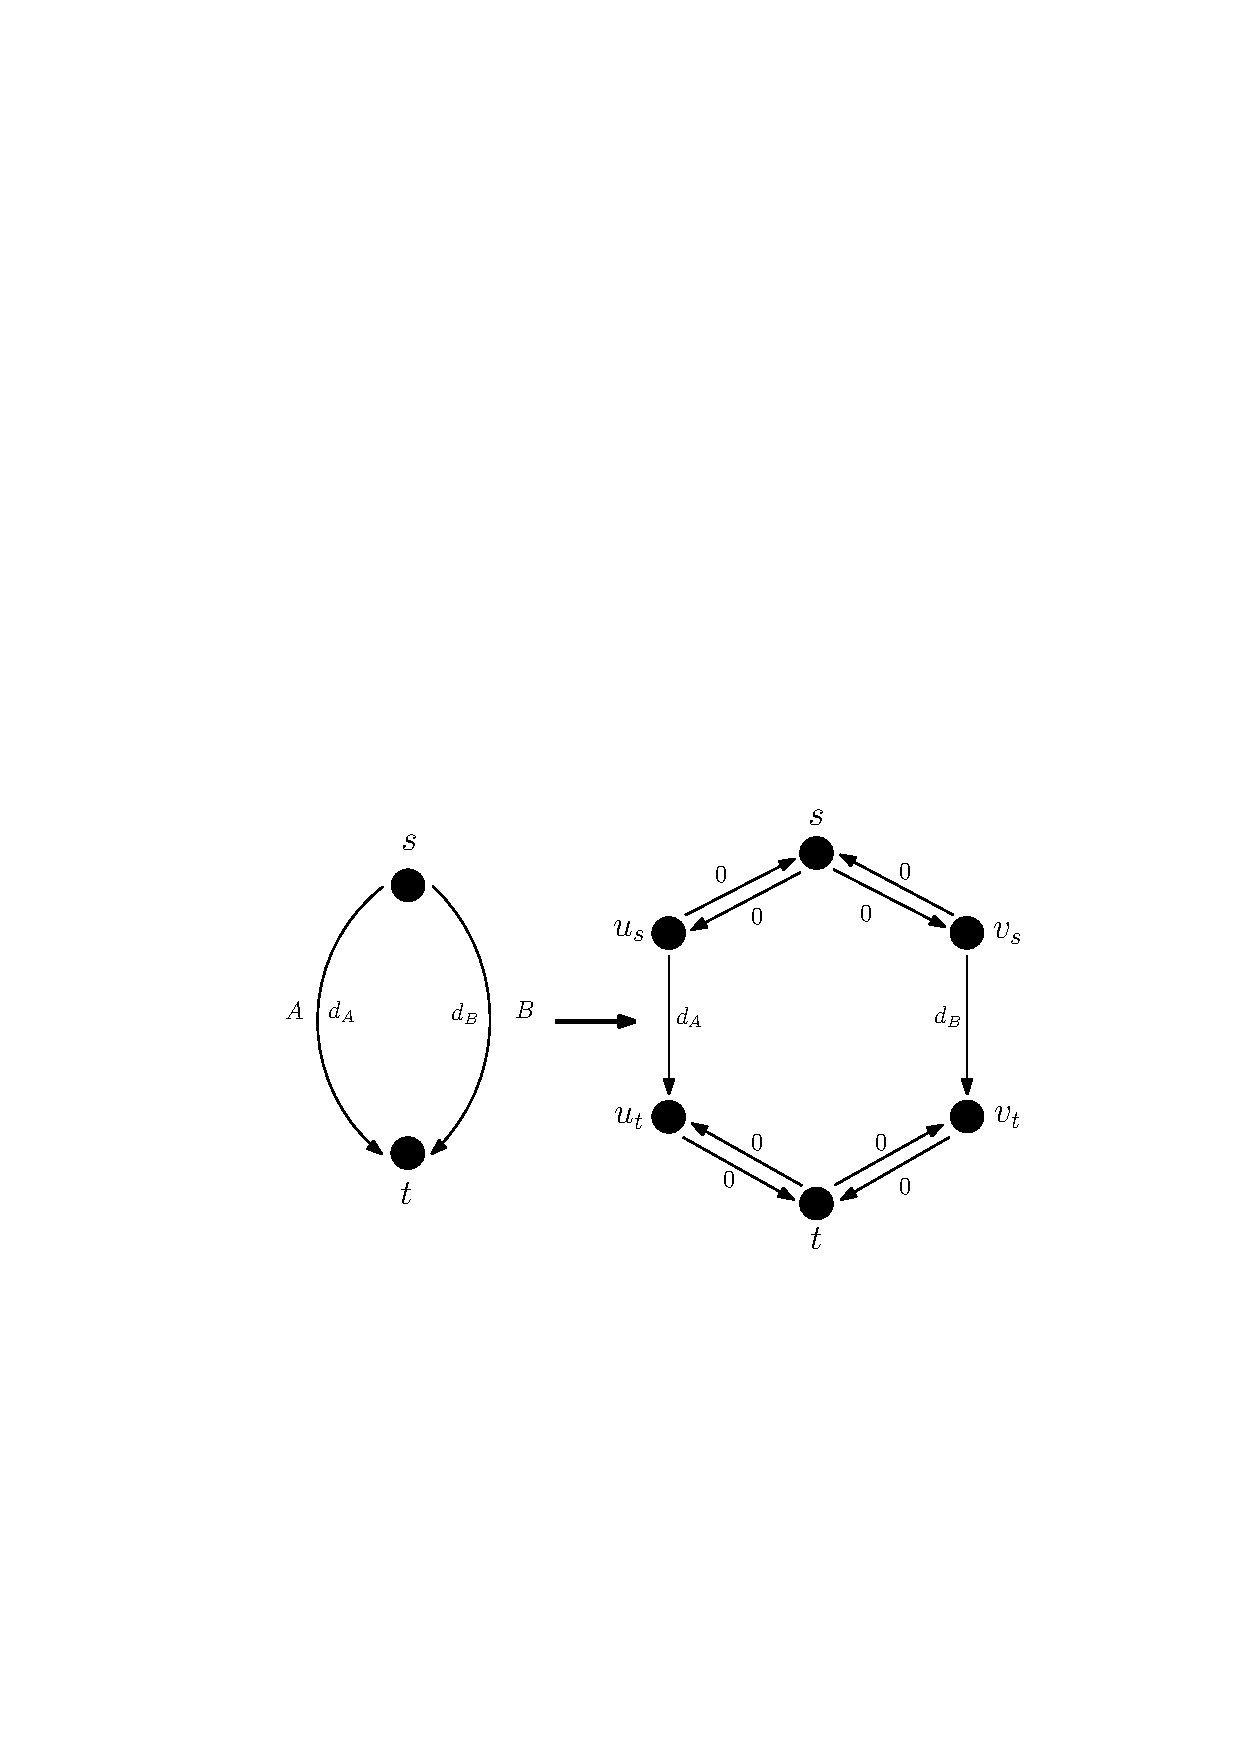
\includegraphics[width = 0.5\textwidth]{images_locomotive/Figure5a.pdf}\label{fig:Figure5a}}\hspace{15pt}
    \subfigure[Transformation for free-move network]{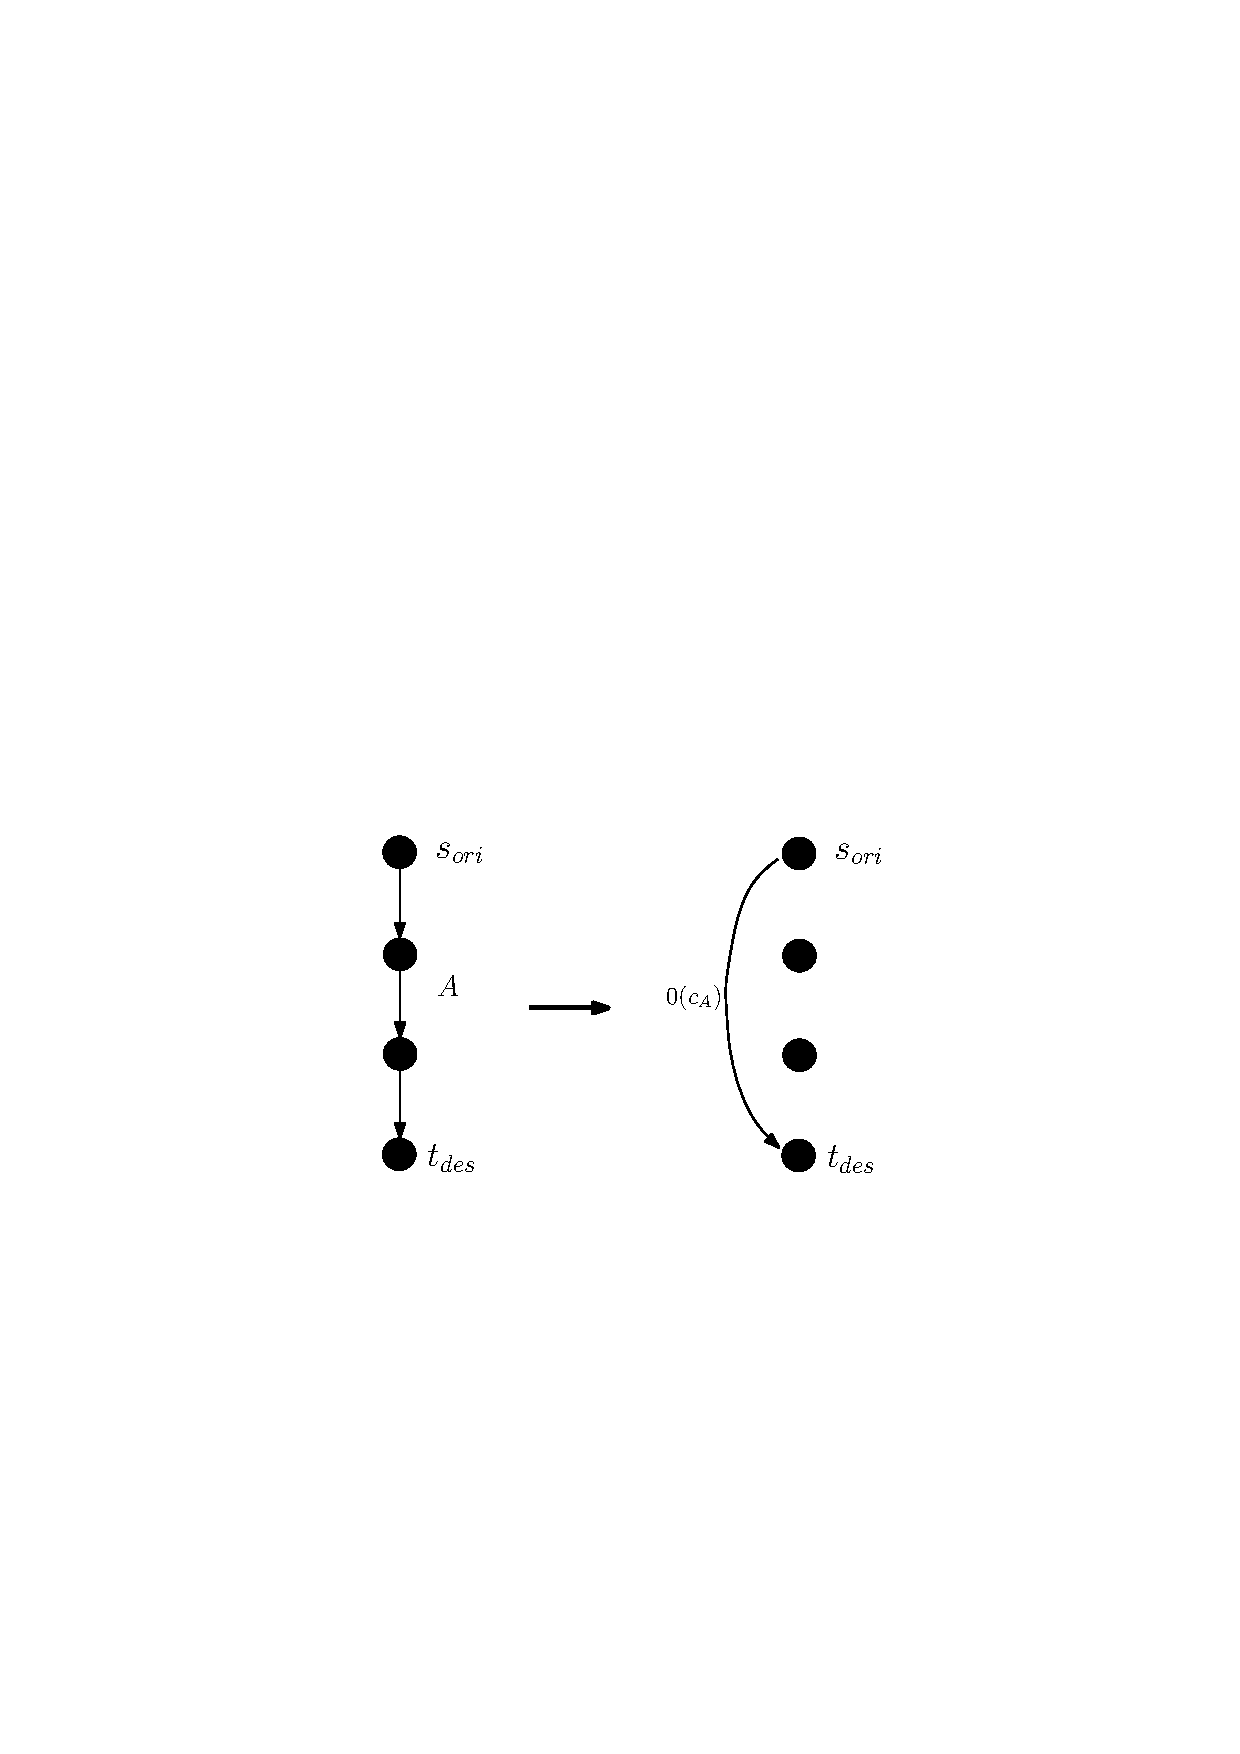
\includegraphics[width=0.4\textwidth]{images_locomotive/Figure5b.pdf}\label{fig:Figure5b}}
    \caption{The two figures illustrate how we transform train network and free-move network by adding new nodes and new edges.}
    \label{fig:Figure5}
\end{figure}


\section{Field Implementation}\label{sec:locomotive:implementation}

We implemented the presented algorithm in C\# on a computer with a three-GHz CPU and four GB of RAM.

\setcounter{table}{1}
\begin{table}[!ht]
 \centering
  \begin{tabular}{cccccccc}
    \hline
        \multirow{2}{*}{Cost} && \multirow{2}{*}{total} & \multirow{2}{*}{capacity}  & locomotive  & \multirow{2}{*}{truck} & regular  & vendor\\
        & &  &   & shipping  &   & fueling & fueling\\
    \hline
        Change ($10^6$ \$) && -72.25 & -0.68  & -109.34  & 36.02  & -7.40  & 6.75 \\
    \hline
   \end{tabular}%
  \caption{We summarize our comparison of the clean-slate scenario and base-case solutions.}%
  \label{tab:Table2}
\end{table}

\begin{table}[!ht]
  \footnotesize
  \centering
  \begin{tabular}{ccccccccc}
    \hline
        &&\multirow{2}{*}{Cost} & \multirow{2}{*}{total} & \multirow{2}{*}{capacity}  & locomotive  & \multirow{2}{*}{truck} & regular  & vendor\\
        &&  &  &   & shipping  &   & fueling & fueling\\
    \hline
        Scenario 1 &&change ($10^6$ \$) & -14.32 & 0.17  & -13.67  & -0.01  & 1.87 & -2.69 \\
    \hline
        Scenario 2 &&change ($10^6$ \$) & -44.90 & 0  & -69.06  & 4.00  & -20.73  & 40.91 \\
    \hline
   \end{tabular}%
  \caption{We summarize our comparison of the incremental scenarios and base-case solutions.}%
  \label{tab:Table3}
\end{table}





